\documentclass[../../main/main.tex]{subfiles}
\graphicspath{{./figures/}}
\usepackage{custikz}

\dominitoc
\faketableofcontents

\renewcommand{\mtcSfont}{\small\bfseries}
\renewcommand{\mtcSSfont}{\footnotesize}
\mtcsettitle{minitoc}{}
\mtcsetrules{*}{off}

\makeatletter
\renewcommand{\@chapapp}{Thermodynamique -- chapitre}
\makeatother

% \toggletrue{student}
% \toggletrue{corrige}
% \renewcommand{\mycol}{black}
% \renewcommand{\mycol}{gray}

\hfuzz=5.003pt

\begin{document}
\setcounter{chapter}{4}

% \settype{book}
% \settype{prof}
% \settype{stud}

\chapter{Machines thermiques}
\epigraph{\openquote\textit{%
		Thermodynamics is a funny subject. The first time you go through it, you
		don't understand it at all. The second time you go through it, you think you
		understand it, except for one or two small points. The third time you go
		through it, you know you don't understand it, but by that time you are so
		used to it, it doesn't bother you anymore.
	}%
	\closequote}{Arnold \textsc{Sommerfeld}, \~1950}

\vspace*{\fill}

\begin{tcn}*(appl)<ctc>{\iconsomm~Sommaire}
	\let\item\olditem
	\vspace{-15pt}
	\minitoc
	\vspace{-25pt}
\end{tcn}

\begin{tcn}*[fontupper=\small](appl)<ctb>"how"'t'{Capacités exigibles}
	\begin{itemize}[label=\rcheck]
		\item Donner le sens des échanges énergétiques pour un moteur ou un
		      récepteur thermique ditherme.

		\item Analyser un dispositif concret et le modéliser par une machine
		      cyclique ditherme.

		\item Définir un rendement ou une efficacité et les relier aux énergies
		      échangées au cours d'un cycle.

		\item Justifier et utiliser le théorème de Carnot.

		\item Citer quelques ordres de grandeur des rendements des machines
		      thermiques réelles actuelles.

		\item Expliquer le principe de la cogénération.
	\end{itemize}
\end{tcn}

\vspace*{\fill}

\newpage

\vspace*{\fill}
% {
% \begin{boxes}
\begin{tcn}[sidebyside, fontupper=\small, fontlower=\small](appl)<ctb>"check"'t'{L'essentiel}
	\begin{tcn}(defi)<ctc>'t'{Définitions}
		\tcblistof[\paragraph*]{defi}{\hspace*{4.8pt}}
	\end{tcn}
	% \begin{tcn}(rapp)<ctc>'t'{Rappels}
	% 	\tcblistof[\paragraph*]{rapp}{\hspace*{4.8pt}}
	% \end{tcn}
	\begin{tcn}(prop)<ctc>'t'{Propriétés}
		\tcblistof[\paragraph*]{prop}{\hspace*{4.8pt}}
		\tcblistof[\paragraph*]{loi}{\hspace*{4.8pt}}
		% \tcblistof[\paragraph*]{theo}{\hspace*{4.8pt}}
	\end{tcn}
	% \begin{tcn}(coro)<ctc>'t'{Corollaires}
	%   \tcblistof[\paragraph*]{coro}{\hspace*{4.8pt}}
	% \end{tcn}
	\begin{tcn}(demo)<ctc>'t'{Démonstrations}
		\tcblistof[\paragraph*]{demo}{\hspace*{4.8pt}}
		\tcblistof[\paragraph*]{prev}{\hspace*{4.8pt}}
	\end{tcn}
	\begin{tcn}(inte)<ctc>'t'{Interprétations}
		\tcblistof[\paragraph*]{inte}{\hspace*{4.8pt}}
	\end{tcn}
	% \begin{tcn}(impl)<ctc>'t'{Implications}
	% 	\tcblistof[\paragraph*]{impl}{\hspace*{4.8pt}}
	% \end{tcn}
	% \begin{tcn}(tool)<ctc>'t'{Outils}
	% 	\tcblistof[\paragraph*]{tool}{\hspace*{4.8pt}}
	% \end{tcn}
	% \begin{tcn}(nota)<ctc>'t'{Notations}
	%   \tcblistof[\paragraph*]{nota}{\hspace*{4.8pt}}
	% \end{tcn}
	% \begin{tcn}(appl)<ctc>'t'{Applications}
	%   \tcblistof[\paragraph*]{appl}{\hspace*{4.8pt}}
	% \end{tcn}
	% \begin{tcn}(rema)<ctc>'t'{Remarques}
	%   \tcblistof[\paragraph*]{rema}{\hspace*{4.8pt}}
	% \end{tcn}
	% \begin{tcn}(exem)<ctc>'t'{Exemples}
	%   \tcblistof[\paragraph*]{exem}{\hspace*{4.8pt}}
	% \end{tcn}
	% \begin{tcn}*(ror)<ctc>"hart"'t'{Points importants}
	%   \tcblistof[\paragraph*]{ror}{\hspace*{4.8pt}}
	% \end{tcn}
	% \begin{tcn}(impo)<ctc>'t'{Erreurs communes}
	%   \tcblistof[\paragraph*]{impo}{\hspace*{4.8pt}}
	% \end{tcn}
	\tcblower
	% \begin{tcn}(defi)<ctc>'t'{Définitions}
	%   \tcblistof[\paragraph*]{defi}{\hspace*{4.8pt}}
	% \end{tcn}
	% \begin{tcn}(rapp)<ctc>'t'{Rappels}
	%   \tcblistof[\paragraph*]{rapp}{\hspace*{4.8pt}}
	% \end{tcn}
	% \begin{tcn}(prop)<ctc>'t'{Propriétés}
	%   \tcblistof[\paragraph*]{prop}{\hspace*{4.8pt}}
	%   \tcblistof[\paragraph*]{loi}{\hspace*{4.8pt}}
	%   \tcblistof[\paragraph*]{theo}{\hspace*{4.8pt}}
	% \end{tcn}
	% \begin{tcn}(coro)<ctc>'t'{Corollaires}
	%   \tcblistof[\paragraph*]{coro}{\hspace*{4.8pt}}
	% \end{tcn}
	% \begin{tcn}(demo)<ctc>'t'{Démonstrations}
	% 	\tcblistof[\paragraph*]{demo}{\hspace*{4.8pt}}
	% 	\tcblistof[\paragraph*]{prev}{\hspace*{4.8pt}}
	% \end{tcn}
	% \begin{tcn}(inte)<ctc>'t'{Interprétations}
	% 	\tcblistof[\paragraph*]{inte}{\hspace*{4.8pt}}
	% \end{tcn}
	\begin{tcn}(impl)<ctc>'t'{Implications}
		\tcblistof[\paragraph*]{impl}{\hspace*{4.8pt}}
	\end{tcn}
	% \begin{tcn}(tool)<ctc>'t'{Outils}
	%   \tcblistof[\paragraph*]{tool}{\hspace*{4.8pt}}
	% \end{tcn}
	% \begin{tcn}(nota)<ctc>'t'{Notations}
	%   \tcblistof[\paragraph*]{nota}{\hspace*{4.8pt}}
	% \end{tcn}
	\begin{tcn}(appl)<ctc>'t'{Applications}
		\tcblistof[\paragraph*]{appl}{\hspace*{4.8pt}}
	\end{tcn}
	% \begin{tcn}(rema)<ctc>'t'{Remarques}
	%   \tcblistof[\paragraph*]{rema}{\hspace*{4.8pt}}
	% \end{tcn}
	% \begin{tcn}(exem)<ctc>'t'{Exemples}
	% 	\tcblistof[\paragraph*]{exem}{\hspace*{4.8pt}}
	% \end{tcn}
	\begin{tcn}*(ror)<ctc>"hart"'t'{Points importants}
		\tcblistof[\paragraph*]{ror}{\hspace*{4.8pt}}
	\end{tcn}
	\begin{tcn}(impo)<ctc>'t'{Erreurs communes}
		\tcblistof[\paragraph*]{impo}{\hspace*{4.8pt}}
	\end{tcn}
\end{tcn}
% \end{boxes}
% }%

\vspace*{\fill}
\newpage

\section{Introduction}
\subsection{Définition}

\begin{tcb*}(defi){Machines thermiques et performance}
	\begin{isd}[righthand ratio=.25]
		Une machine thermique est un dispositif qui fait subir à un fluide un
		\textbf{cycle thermodynamique}, dans le but d'\textbf{extraire du travail}
		mécanique $W$ ou un \textbf{transfert thermique} $Q$.
		% Selon le type de machine, l'énergie coûteuse et l'énergie produite ne sont pas
		% les mêmes.
		\tcblower
		\tcbsubtitle{\fatbox{\textbf{Coeff.\ performance}}}
		\vspace{-15pt}
		\psw{%
			\[
				\text{COP} = \abs{\frac{\text{production}}{\text{coût}}}
			\]
		}%
		\vspace{-15pt}
	\end{isd}
	\begin{isd}[sidebyside align=top]
		\tcbsubtitle{\fatbox{\textbf{Machine motrice}}}
		Elle \textbf{fournit un travail}~:
		\begin{itemize}
			\item[b]{Production}: \psw{$W < 0$}
			\item[b]{Coût}: \psw{$Q > 0$}
			\item[b]{Rendement}\ftn{On parle de \textbf{rendement} pour un
				\textbf{moteur}, car il décrit une conversion d'énergie. On a donc
				$\eta < 1$.}: \psw{$\DS\eta = \abs{\frac{W}{Q}}$}
		\end{itemize}
		\vspace{-15pt}
		\tcblower
		\tcbsubtitle{\fatbox{\textbf{Machine réceptrice}}}
		Elle \textbf{reçoit un travail}~:
		\begin{itemize}
			\item[b]{Coût}: \psw{$W > 0$}
			\item[b]{Production}: \psw{$Q \lessgtr 0$}
			\item[b]{Efficacité}\ftn{On parle d'\textbf{efficacité} pour un
				\textbf{récepteur} puisqu'elle quantifie un transfert thermique, pas
				une conversion. On peut donc avoir $e > 1$.}: \psw{$\DS e =
					\abs{\frac{Q}{W}}$}
		\end{itemize}
		\vspace{-15pt}
	\end{isd}
\end{tcb*}
\vspace{-15pt}
\begin{tcb}(exem)<lftt>{Machines thermiques}
	\begin{itemize}
		\item Une locomotive à vapeur convertit la chaleur extraite de la cheminée
		      en mouvement des roues~: c'est un \xul{\psw{\textbf{moteur}}}.
		\item Un radiateur électrique convertit un travail électrique (effet
		      \textsc{Joule}) en chaleur~: c'est un \xul{\psw{\textbf{récepteur}}}.
		\item Un réfrigérateur récupère un travail électrique et s'en sert pour
		      capter l'énergie thermique des aliments~: c'est un
		      \xul{\psw{\text{récepteur}}}.
	\end{itemize}
\end{tcb}

\vspace{-25pt}
\subsection{Fonctionnement général}
\begin{tcb*}[sidebyside](prop){Fonctionnement des machines thermiques}
	Pour une machine en contact avec $n$ sources de chaleurs, son fonctionnement
	est régit par les \textbf{deux principes} de la thermodynamique~:
	\begin{itemize}
		\item[b]{Premier principe}:
		\psw{%
			\[
				\boxed{W + \sum_{i=1}^{n} Q_i = 0}
			\]
		}%
		\vspace{-15pt}
		\item[b]{Second principe} (\textbf{inégalité de \textsc{Clausius}}):
		\psw{%
			\[
				\boxed{\sum_{i=1}^{n} \frac{Q_i}{T_i} \leq 0}
			\]
		}%
		% Qu'on appelle aussi \textbf{inégalité de \textsc{Clausius}}
	\end{itemize}
	\tcblower
	\begin{center}
		\sswitch{
			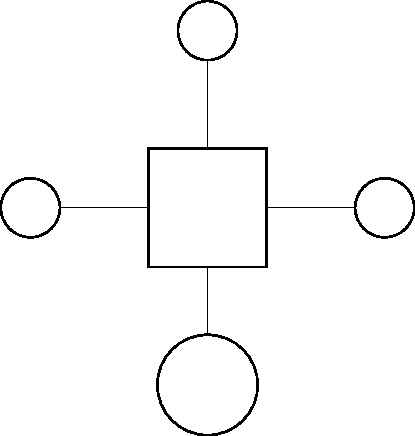
\includegraphics[scale=.8]{ppe_gen-stud}
		}{
			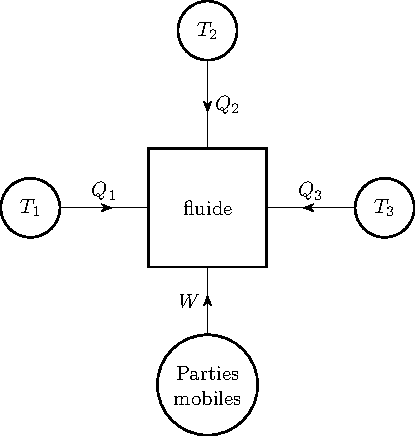
\includegraphics[scale=.8]{ppe_gen}
		}
		\captionof{figure}{Représentation des échanges}
	\end{center}
\end{tcb*}

\begin{tcb*}(impo){Échanges algébriques}
	Pour rappel, les énergies échangées sont \textbf{algébriques}, et dans le
	premier principe $W$ et $Q$ sont des énergies \textbf{reçues}~: les flèches
	sont donc dirigées \textbf{vers le fluide}, même si les échanges sont
	négatifs. On indiquera explicitement le signe des échanges pour lever la
	confusion selon le type de machine.
\end{tcb*}

\begin{tcb*}[sidebyside, sidebyside align=top](demo){Fonctionnement des machines thermiques}
	\tcbsubtitle{\fatbox{\textbf{Premier principe}}}
	\vspace{-15pt}
	\psw{%
		\begin{align*}
			\Delta{U}\ind{cycle} & = 0
			\\\Lra
			W + \sum_i Q_i       & = 0
			\\\Lra
			\Aboxed{\sum_i Q_i   & = -W}
			\qed
		\end{align*}
	}%
	\vspace{-15pt}
	\tcblower
	\tcbsubtitle{\fatbox{\textbf{Inégalité de \textsc{Clausius}}}}
	\vspace{-15pt}
	\psw{%
		\begin{align*}
			\Delta{S}\ind{cycle}                                               & = 0
			\\\Lra
			\sum_i S_{\mathrm{ech},i} + \underbracket[1pt]{S\ind{cr}}_{\geq 0} & = 0
			\\\Lra
			\Aboxed{
			\sum_{i=1}^{n} \frac{Q_i}{T_i}                                     & \leq 0
			}
			\qed
		\end{align*}
	}%
	\vspace{-15pt}
\end{tcb*}

\subsection{Machines monothermes}
\begin{tcb*}(defi){Machine monotherme}
	Une machine thermique monotherme est composée d'un fluide en contact avec un
	\textbf{unique thermostat}.
\end{tcb*}


\end{document}

% \begin{center}
% 	\begin{tikzpicture}[scale=1.3]
% 		\draw [->](0,0) -- (0,3.5) node[anchor=west]{$P$};
% 		\draw [->](0,0) -- (5.5,0) node[anchor=west]{$V$};
%
% 		\draw[dashed] plot [domain=0.8:5] (\x,3/\x) node[below]{$T_f$};
% 		\draw[very thick, red,simplef] plot [domain=1.5:3] (\x,3/\x);
% 		\draw[very thick, red,simplef] plot [domain=1.0203:1.5] (\x,{3.5282/(\x^(1.4))});
% 		\draw[dashed] plot [domain=0.8:5] (\x,3.5/\x) node[above]{$T_c$};
% 		\draw[very thick, red,simplef] plot [domain=2.0406:1.0203] (\x,3.5/\x);
% 		\draw[very thick, red,simplef] plot [domain=3:2.0406] (\x,{4.6555/(\x^(1.4))});
%
% 		\fill (3,1) circle(0.04);
% 		\fill (1.5,2) circle(0.04);
% 		\fill (1.0203,3.43) circle(0.04);
% 		\fill (2.0406,1.72) circle(0.04);
%
% 		\node[above] at (3,1) {A};
% 		\node[left] at (1.5,2) {D};
% 		\node[right] at (1.0203,3.43) {C};
% 		\node[right] at (2.0406,1.72) {B};
% 	\end{tikzpicture}
% \end{center}
